\begin{figure}[htp]
  \centering
  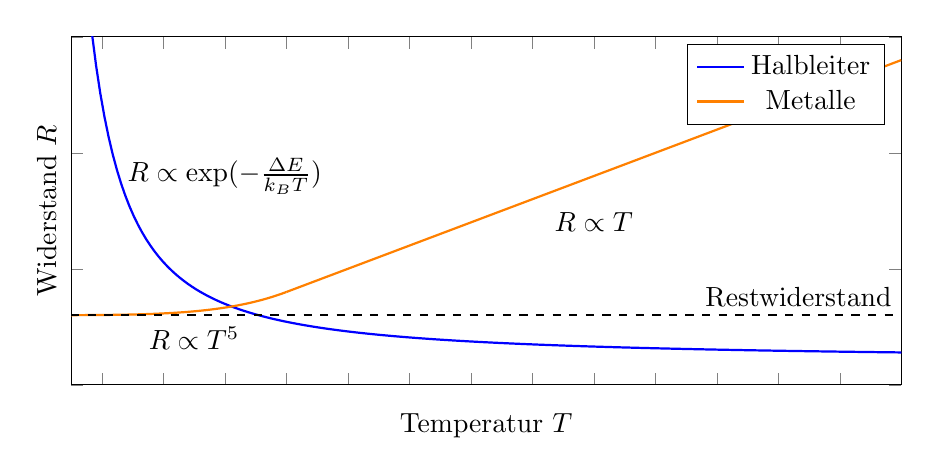
\begin{tikzpicture}[every text node part/.style={align=center}]
    \begin{axis}[disabledatascaling, width=\textwidth, height=6cm, ylabel=Widerstand $R$, xlabel=Temperatur $T$, xmin=3, xmax=30, ymin = 0, ymax = 15, samples = 200, xticklabels={}, yticklabels={}, y label style={yshift=-.5em}]
      \addplot[blue, thick, domain = 3:30] {exp(10/x};
      \addlegendentry{Halbleiter}
      \addplot[orange, thick, domain = 0:10] {0.00001*(x)^5+3};
      \addplot[orange, thick, domain = 10:30] {0.5*(x-10)+4};
      \addlegendentry{Metalle}
      \draw[dashed, thick] (3,3) -- (30,3);
      \node[anchor=east] (A) at (30,3.8){Restwiderstand};
      \node (A) at (20,7){$R \propto T$};
      \node (A) at (7,2){$R \propto T^5$};
      \node (A) at (8,9){$R \propto \exp\qty(-\frac{\Delta E}{k_B T})$};
    \end{axis}
\end{tikzpicture}
  \caption{Schematische Darstellung der Temperaturabhängigkeit des elektrischen Widerstands für Metalle und Halbleiter.}
  \label{fig:Elektrischer_Widerstand}
\end{figure}
